%#########################################################################
\chapter{Interferencia y Difracción}
\label{cha:optic}


%#########################################################################



%*************************************************************************
\section{Demostración 1: Interferencia por reflexión}
\label{sec:DEMO4_01}
\rule{14cm}{0.5mm}

Como se ha mencionado al inicio de estas guías, el objetivo es introducir 
progresivamente herramientas de programación más avanzadas y útiles para
el desarrollo de códigos de diferente índole. Se pretende lograr este 
objetivo usando los temas del curso de Oscilaciones y Ondas.

\
%.........................................................................
%Interference
\begin{figure}[htbp]
	\centering
	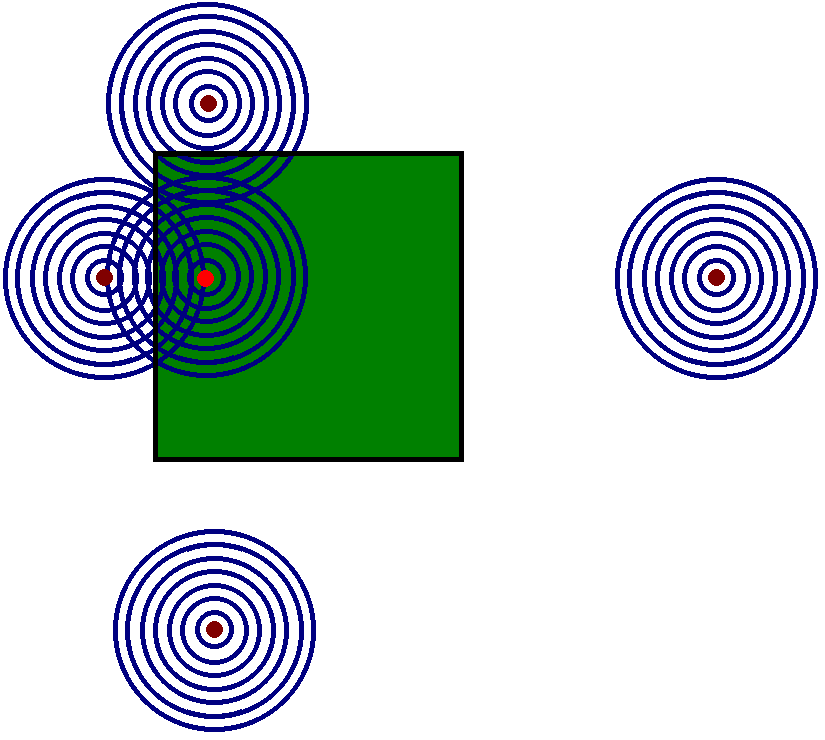
\includegraphics[width=0.62\textwidth]
	{./pictures/sound_interference.png}

	\caption{\small{Interferencia por reflexión.}}
	
	\label{fig:reflex_interference}
\end{figure}
%.........................................................................


En esta demostración se usará una herramienta para el desarrollo de 
interfaces gráficas en \python llamada \textit{Tkinter}. Esta librería es
de uso estándar en \python y viene precargada, así que no requiere de 
instalación previa. El objetivo de la demostración es calcular el patrón 
de interferencia de una onda sonora en un cuarto cuadrado producido por la
reflexión en las paredes. Posteriormente se simula el sonido captado por
un observador ubicado en una posición dada dentro del cuarto.

\

Por simplicidad se describirá la oscilación producida por las fuentes 
como una onda radial de la forma

%.........................................................................
%Radial wave
\eq{eq:radial_wave}
{z(r, t) = \frac{A_0}{1+r}\sin\pr{\omega t - k r } = 
A_0\sin\cor{2\pi \pr{\frac{t}{f} - \frac{r}{\lambda} }}}
%.........................................................................

donde $z(r, t)$ es la función de amplitud en $z$ de la onda, $A_0$ la 
amplitud máxima del desplazamiento, $\omega$ la frecuencia angular, $f$ la 
frecuencia y $\lambda$ la longitud de onda. El valor de $r$ es medido 
desde el origen de la perturbación, es decir, en la posición de cada fuente.
Para calcular la amplitud total se usa el principio de superposición, donde
se suman las contribuciones de la fuente original y las 4 fuentes imágenes
que simulan la reflexión. Además, a partir de la ley de conservación de
energía, se usa un decaimiento como $1/r$ en la amplitud, con un tamaño 
asociado de la fuente de $1$ m.

\

A continuación de ilustra el código de la demostración


%ccccccccccccccccccccccccccccccccccccccccccccccccccccccccccccccccccccccccc
%DEMO 5_01
\begin{listing}[style=python]
#!/usr/bin/env python
#==========================================================
# DEMOSTRACION 1:
# Simulacion de interferencia en una caja cuadrada
#==========================================================

import AudioLib as ad
import Tkinter
import matplotlib.pylab as plt
import numpy as np
import scipy.interpolate as interp

from matplotlib.backends.backend_tkagg \
import FigureCanvasTkAgg, NavigationToolbar2TkAgg
from matplotlib.figure import Figure

#Funcion de amplitud de una fuente
def Z_amplitud(x, y, x0, y0, t, f, lamb):
    #Posicion de la fuente
    r0 = np.array([x0, y0])
    #Posicion donde se evalua el campo
    r = np.array([x, y])
    rr0 = np.linalg.norm(r-r0)
    return ad.Amplitude*1/(rr0+1.0)*\
    np.sin( 2*np.pi*(t*f - rr0/lamb ) )

#==========================================================
# Clase App para la generacion de entorno grafico
#==========================================================
class App:
  def __init__(self, master):
    #Creando contenedor
    self.frame = Tkinter.Frame(master)
    #******************************************************
    #	Propiedades Fuente
    #******************************************************
    #Etiqueta de Propiedades de la Fuente
    self.label = Tkinter.Label(self.frame,\
    text='PROPIEDADES\n DE LA FUENTE')
    self.label.pack(side='top')
    
    #Tamano caja
    self.label = Tkinter.Label(self.frame,\
    text='Longitud Caja [m]')
    self.label.pack(side='top') 
    self.Lbox = Tkinter.DoubleVar()
    self.L_textbox = Tkinter.Entry( self.frame,\
    textvariable = self.Lbox, width = 6 )
    self.L_textbox.pack(side='top')

    #Coordenada x
    self.label = Tkinter.Label(self.frame, text='X')
    self.label.pack(side='top') 
    self.xsource = Tkinter.DoubleVar()
    self.xs_textbox = Tkinter.Entry( self.frame,\
    textvariable = self.xsource, width = 6 )
    self.xs_textbox.pack(side='top')
    
    #Coordenada y
    self.label = Tkinter.Label(self.frame, text='Y')
    self.label.pack(side='top') 
    self.ysource = Tkinter.DoubleVar()
    self.ys_textbox = Tkinter.Entry( self.frame,\
    textvariable = self.ysource, width = 6 )
    self.ys_textbox.pack(side='top')
        
    #Velocidad onda
    self.label = Tkinter.Label(self.frame,\
    text='Velocidad Onda [m/s]')
    self.label.pack(side='top') 
    self.vel = Tkinter.DoubleVar()
    self.vel_textbox = Tkinter.Entry( self.frame,\
    textvariable = self.vel, width = 6 )
    self.vel_textbox.pack(side='top')

    #Frecuencia de onda
    self.label = Tkinter.Label(self.frame,\
    text='Frecuencia [Hz]')
    self.label.pack(side='top') 
    self.freq = Tkinter.DoubleVar()
    self.f_textbox = Tkinter.Entry( self.frame,\
    textvariable = self.freq, width = 6 )
    self.f_textbox.pack(side='top')
    
    #Seleccion de condiciones de frontera
    self.label = Tkinter.Label(self.frame,\
    text='Frontera reflectiva\n[0 -- no\t1 -- si]')
    self.label.pack(side='top')  
    self.frontera = Tkinter.IntVar()
    self.front_textbox = Tkinter.Entry( self.frame,\
    textvariable = self.frontera, width = 6 )
    self.front_textbox.pack(side='top')
    
    #Boton Calcular fuente
    self.sour_buttom = Tkinter.Button( self.frame,\
    text="Calcular Fuente", command=self.plot_source,\
    width =12)
    self.sour_buttom.pack(side = 'top')
        
        
    #******************************************************
    #	Propiedades Observador
    #******************************************************
    #Etiqueta de Propiedades del obsevador
    self.label = Tkinter.Label(self.frame,\
    text='PROPIEDADES\n DEL OBSERVADOR')
    self.label.pack(side='top')
    
    #Coordenada x
    self.label = Tkinter.Label(self.frame, text='X')
    self.label.pack(side='top') 
    self.xobs = Tkinter.DoubleVar()
    self.xo_textbox = Tkinter.Entry( self.frame,\
    textvariable = self.xobs, width = 6 )
    self.xo_textbox.pack(side='top')
    
    #Coordenada y
    self.label = Tkinter.Label(self.frame, text='Y')
    self.label.pack(side='top') 
    self.yobs = Tkinter.DoubleVar()
    self.yo_textbox = Tkinter.Entry( self.frame,\
    textvariable = self.yobs, width = 6 )
    self.yo_textbox.pack(side='top')
    
    #Tiempo senal
    self.label = Tkinter.Label(self.frame,\
    text='Tiempo observador')
    self.label.pack(side='top') 
    self.tmax = Tkinter.DoubleVar()
    self.tm_textbox = Tkinter.Entry( self.frame,\
    textvariable = self.tmax, width = 6 )
    self.tm_textbox.pack(side='top')
    
    #Boton Calcular Audio
    self.obs_buttom = Tkinter.Button( self.frame,\
    text="Calcular Audio", command=self.plot_obs,\
    width =12)
    self.obs_buttom.pack(side = 'top')

    fig = Figure(figsize=(6,6))
    self.ax = fig.add_subplot(111)
    self.ax.set_title("Interferencia",\
    fontsize=15)
    self.canvas = FigureCanvasTkAgg(fig,master=master)
    self.ax.grid()
    self.canvas.show()
    self.canvas.get_tk_widget().pack(side='right',\
    fill='none', expand=0)
    self.frame.pack()

  #******************************************************
  #	General Properties Methods
  #******************************************************
  #Grafiacion del campo
  def plot_source(self):
    #Tamano caja
    L = self.Lbox.get()
    #Resolucion de la caja
    NS = 200
    #Grid
    XM = np.linspace( 0, L, NS )
    YM = np.linspace( 0, L, NS )
    #Posicion de la fuente
    X0 = self.xsource.get()
    Y0 = self.ysource.get()
    #Frecuencia
    f = self.freq.get()
    #Velocidad de onda
    vel = self.vel.get()
    #Longitud de onda
    lamb = vel/f
    #Condicional de fronteras reflectivas
    reflex = self.frontera.get()
    
    #Calculo de Amplitud del campo
    Z = np.zeros( (NS,NS) )
    for i in xrange( 0, NS ):
      for j in xrange( 0, NS ):
	x = XM[i]
	y = YM[j]
	Z[-j,i] = \
	Z_amplitud(x, y, X0, Y0, 0.0, f, lamb )
	if reflex == 1:
	  Z[-j,i] -= \
	  Z_amplitud(x, y, 0.0, -Y0, 0.0, f, lamb ) +\
	  Z_amplitud(x, y, 0.0, 2*L-Y0, 0.0, f, lamb ) +\
	  Z_amplitud(x, y, -X0, 0.0, 0.0, f, lamb ) +\
	  Z_amplitud(x, y, 2*L-X0, 0.0, 0.0, f, lamb )

    self.ax.clear()
    self.ax.grid()
    self.ax.set_title('Amplitud Onda Sonora')
    self.ax.set_xlabel('X [m]')
    self.ax.set_ylabel('Y [m]')
    self.ax.imshow( Z, extent = (0,L,0,L) )
    self.canvas.draw()
    
    
  #Grafiacion del sonido medido por el observador
  def plot_obs(self):
    #Tamano caja
    L = self.Lbox.get()
    #Posicion de la fuente
    X0 = self.xsource.get()
    Y0 = self.ysource.get()
    #Posicion del observador
    XOb = self.xobs.get()
    YOb = self.yobs.get()
    #Frecuencia
    f = self.freq.get()
    #Velocidad de onda
    vel = self.vel.get()
    #Longitud de onda
    lamb = vel/f
    #Condicional de fronteras reflectivas
    reflex = self.frontera.get()
    
    #Intervalo de tiempo
    dt = 1/(44100.)
    #Tiempo maximo
    tmax = self.tmax.get()
    #Arreglo de tiempo
    self.tiempo = np.arange( 0, tmax, dt )
    #Calculo de campo en el punto del observador
    self.Z = \
    Z_amplitud(XOb, YOb, X0, Y0, self.tiempo, f, lamb )
    if reflex == 1:
      self.Z -= \
      Z_amplitud(XOb,YOb,0.0,-Y0,self.tiempo,f,lamb)+\
      Z_amplitud(XOb,YOb,0.0,2*L-Y0,self.tiempo,f,lamb)+\
      Z_amplitud(XOb,YOb,-X0,0.0,self.tiempo,f,lamb)+\
      Z_amplitud(XOb,YOb,2*L-X0,0.0,self.tiempo,f,lamb)
      self.Z *= 1/(5.)
    #Grafica
    self.ax.clear()
    self.ax.grid()
    self.ax.set_title('Amplitud Onda Sonora por Observador')
    self.ax.set_xlabel('tiempo [s]')
    self.ax.set_ylabel('Amplitud [$A_0$]')
    self.ax.plot( self.tiempo, self.Z/(1.0*ad.Amplitude) )
    self.ax.set_ylim( (-1, 1) )
    self.ax.set_xlim( (0, tmax) )
    self.canvas.draw()
    #Creando objeto de audio
    sonido = ad.audio()
    #Cargando nota de audio
    sonido.load( self.Z )
    #Reproduciendo sonido
    sonido.play()
        
root = Tkinter.Tk()
root.wm_title("Interferencia Sonora")
app = App(root)
root.mainloop()
\end{listing}
%ccccccccccccccccccccccccccccccccccccccccccccccccccccccccccccccccccccccccc

El resultado obtenido es una interfaz gráfica que permite la interacción 
dinámica con el usuario.


%.........................................................................
%Environment Initially
\begin{figure}[htbp]
	\centering
	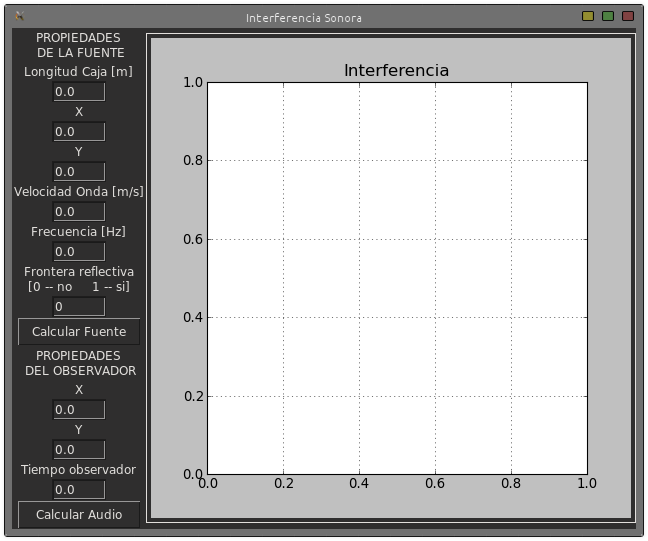
\includegraphics[width=0.60\textwidth]
	{./pictures/environment_Initial.png}

	\caption{\small{Entorno gráfico: ventana inicial.}}
	
	\label{fig:env_empty}
\end{figure}
%.........................................................................

%.........................................................................
%Environment Field
\begin{figure}[htbp]
	\centering
	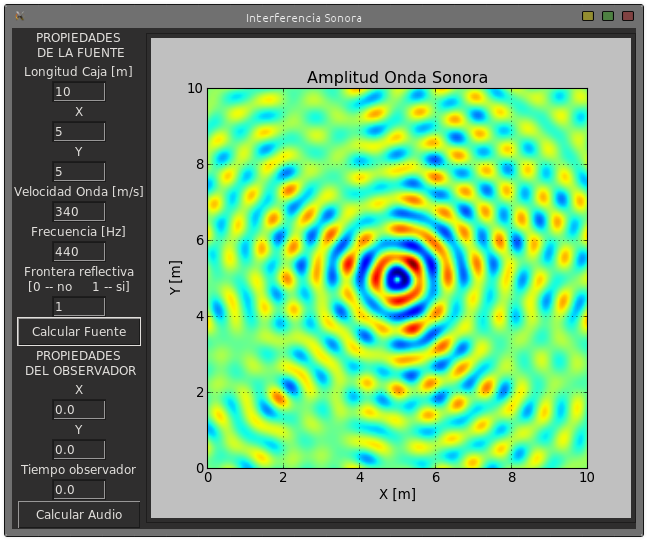
\includegraphics[width=0.60\textwidth]
	{./pictures/environment_field.png}

	\caption{\small{Entorno gráfico: cálculo del campo de interferencia.}}
	
	\label{fig:env_field}
\end{figure}
%.........................................................................

%.........................................................................
%Environment Sound
\begin{figure}[htbp]
	\centering
	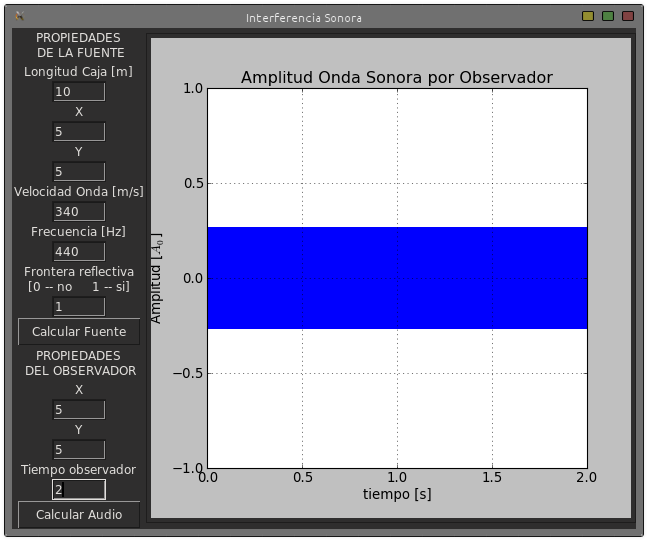
\includegraphics[width=0.60\textwidth]
	{./pictures/environment_sound.png}

	\caption{\small{Entorno gráfico: cálculo del audio percibido por el \
	observador.}}
	
	\label{fig:env_soun}
\end{figure}
%.........................................................................


A continuación se explica cada parte del código


%ccccccccccccccccccccccccccccccccccccccccccccccccccccccccccccccccccccccccc
%DEMO 5_01
\begin{listing}[style=python, numbers = none]
import AudioLib as ad
import Tkinter
import matplotlib.pylab as plt
import numpy as np

from matplotlib.backends.backend_tkagg \
import FigureCanvasTkAgg, NavigationToolbar2TkAgg
from matplotlib.figure import Figure
\end{listing}
%ccccccccccccccccccccccccccccccccccccccccccccccccccccccccccccccccccccccccc
Además de las librerías estándar ya conocidas, se cargan las librerías 
\texttt{AudioLib}, para el manejo de los objetos de audio y \texttt{Tkinter}
para usar las funciones que permiten construir el entorno gráfico. En las 
últimas dos líneas se cargan funciones especificas que permiten embeber
entornos de graficación en el entorno gráfico global.
 

%ccccccccccccccccccccccccccccccccccccccccccccccccccccccccccccccccccccccccc
%DEMO 5_01
\begin{listing}[style=python, numbers = none]
#Funcion de amplitud de una fuente
def Z_amplitud(x, y, x0, y0, t, f, lamb):
    #Posicion de la fuente
    r0 = np.array([x0, y0])
    #Posicion donde se evalua el campo
    r = np.array([x, y])
    rr0 = np.linalg.norm(r-r0)
    return ad.Amplitude*1/(rr0+1.0)*\
    np.sin( 2*np.pi*(t*f - rr0/lamb ) )
\end{listing}
%ccccccccccccccccccccccccccccccccccccccccccccccccccccccccccccccccccccccccc
Se define la función de amplitud para una fuente puntual. Los argumentos
son, la coordenada del punto donde se desea evaluar el campo (\texttt{x},
\texttt{y}), la coordenada de la fuente (\texttt{x0}, \texttt{y0}), el 
tiempo actual \texttt{t}, la frecuencia \texttt{f} y la longitud de 
\texttt{onda}. La amplitud se toma como el máximo valor que puede registrar
un computador en volumen\footnote{Este valor está almacenado en la librería
\texttt{AudioLib} y se accede como \texttt{ad.Amplitude}}


%ccccccccccccccccccccccccccccccccccccccccccccccccccccccccccccccccccccccccc
%DEMO 5_01
\begin{listing}[style=python, numbers = none]
#==========================================================
# Clase App para la generacion de entorno grafico
#==========================================================
class App:
  def __init__(self, master):
    #Creando contenedor
    self.frame = Tkinter.Frame(master)
    #******************************************************
    #	Propiedades Fuente
    #******************************************************
    #Etiqueta de Propiedades de la Fuente
    self.label = Tkinter.Label(self.frame,\
    text='PROPIEDADES\n DE LA FUENTE')
    self.label.pack(side='top')
\end{listing}
%ccccccccccccccccccccccccccccccccccccccccccccccccccccccccccccccccccccccccc
En esta parte se crea un objeto llamado \texttt{App} que contiene toda la 
información asociada al entorno gráfico. Esta parte es genérica y es 
usada para la creación de cualquier entorno con \texttt{Tkinter}.


Se define la función \texttt{\_\_init\_\_} que inicializa la clase 
\texttt{App}, \texttt{def \_\_init\_\_(self, master):}. Su función 
específica es inicializar el entorno.


Con \texttt{self.frame = Tkinter.Frame(master)} se crea un marco vacío
para embeber todos los elementos gráficos. Con la función 
\texttt{Tkinter.Label} se crea una etiqueta con el nombre \texttt{"PROPIEDADES
DE LA FUENTE"} y finalmente con \texttt{self.label.pack} se posiciona el
elemento tipo label en la interfaz gráfica, especificando \texttt{"top"}
como la posición donde será ubicado.

%.........................................................................
%Environment label1
\begin{figure}[htbp]
	\centering
	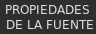
\includegraphics[width=0.10\textwidth]
	{./pictures/environment_label1.png}
	\label{fig:env_label1}
\end{figure}
%.........................................................................


%ccccccccccccccccccccccccccccccccccccccccccccccccccccccccccccccccccccccccc
%DEMO 5_01
\begin{listing}[style=python, numbers = none]
    #Tamano caja
    self.label = Tkinter.Label(self.frame,\
    text='Longitud Caja [m]')
    self.label.pack(side='top') 
    self.Lbox = Tkinter.DoubleVar()
    self.L_textbox = Tkinter.Entry( self.frame,\
    textvariable = self.Lbox, width = 6 )
    self.L_textbox.pack(side='top')
\end{listing}
%ccccccccccccccccccccccccccccccccccccccccccccccccccccccccccccccccccccccccc
Se crea nuevamente una etiqueta con el nombre de \texttt{"Longitud Caja [m]"}
y se posiciona en la parte superior disponible. Ahora, con en la línea
\texttt{self.Lbox = Tkinter.DoubleVar()} se crea la variable tipo double 
\texttt{Lbox}, la cual sirve para almacenar el valor dado por el usuario 
para el tamaño de la caja. Finalmente usando la función \texttt{Tkinter.Entry}
se crea una caja de texto para la interacción con el usuario, como 
argumentos se tiene, el marco donde quiere embeberse el elemento, 
\texttt{self.frame}, la variable donde se almacenará el valor dado 
\texttt{textvariable = self.Lbox} y el tamaño de la caja \texttt{width = 6}.
Luego, usando de nuevo el atributo \texttt{pack}, se ubica el elemento en
la parte superior disponible.

%.........................................................................
%Environment Lbox
\begin{figure}[htbp]
	\centering
	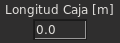
\includegraphics[width=0.15\textwidth]
	{./pictures/environment_Lbox.png}
	\label{fig:env_Lbox}
\end{figure}
%.........................................................................


Se repite el mismo procedimiento para las coordenadas \texttt{X} y \texttt{Y}
de la fuente, la velocidad de la onda, la frecuencia y la condición de 
frontera reflectiva. En este último caso se usa una variable tipo 
\texttt{Tkinter.IntVar()} debido a que la condición de frontera reflectiva
es un booleano que toma los valores \texttt{0} (no reflectiva) o \texttt{1}
(reflectiva).


%.........................................................................
%Environment source
\begin{figure}[htbp]
	\centering
	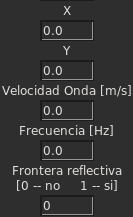
\includegraphics[width=0.15\textwidth]
	{./pictures/environment_source.png}
	\label{fig:env_source}
\end{figure}
%.........................................................................


%ccccccccccccccccccccccccccccccccccccccccccccccccccccccccccccccccccccccccc
%DEMO 5_01
\begin{listing}[style=python, numbers = none]
    #Boton Calcular fuente
    self.sour_buttom = Tkinter.Button( self.frame,\
    text="Calcular Fuente", command=self.plot_source,\
    width = 12)
    self.sour_buttom.pack(side = 'top')
\end{listing}
%ccccccccccccccccccccccccccccccccccccccccccccccccccccccccccccccccccccccccc
Finalmente para la fuente, se define un objeto tipo botón. Para esto se
usa el comando \texttt{Tkinter.Button}, el cual tiene como argumentos el 
marco donde será embebido el objeto, \texttt{self.frame}, el texto del 
botón \texttt{'Calcular Fuente'}, la función que se ejecuta cuando es 
presionado el botón \texttt{command=self.plot\_source} y el tamaño del 
botón \texttt{width = 12}. Luego, usando el método \texttt{pack} se ubica 
el botón en la parte superior disponible.

%.........................................................................
%Environment button 1
\begin{figure}[htbp]
	\centering
	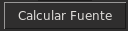
\includegraphics[width=0.15\textwidth]
	{./pictures/environment_button1.png}
	\label{fig:env_button1}
\end{figure}
%.........................................................................


Todo lo anterior se repite para las propiedades del observador

%.........................................................................
%Environment observer
\begin{figure}[htbp]
	\centering
	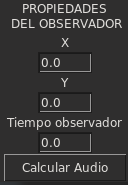
\includegraphics[width=0.15\textwidth]
	{./pictures/environment_obs.png}
	\label{fig:env_obs}
\end{figure}
%.........................................................................

En el caso del observador, el botón \texttt{Calcular Audio} ejecuta la 
función \texttt{plot\_obs}.

%ccccccccccccccccccccccccccccccccccccccccccccccccccccccccccccccccccccccccc
%DEMO 5_01
\begin{listing}[style=python, numbers = none]
    fig = Figure(figsize=(6,6))
    self.ax = fig.add_subplot(111)
    self.ax.set_title("Interferencia",\
    fontsize=15)
    self.canvas = FigureCanvasTkAgg(fig,master=master)
    self.ax.grid()
    self.canvas.show()
    self.canvas.get_tk_widget().pack(side='right',\
    fill='none', expand=0)
    self.frame.pack()
\end{listing}
%ccccccccccccccccccccccccccccccccccccccccccccccccccccccccccccccccccccccccc
Esta parte del código es estándar y sirve para embeber el entorno de 
graficación de \matplotlib en el entorno gráfico.

\

A continuación se explican las funciones definidas, inicialmente la función
\texttt{plot\_source}.


%ccccccccccccccccccccccccccccccccccccccccccccccccccccccccccccccccccccccccc
%DEMO 5_01
\begin{listing}[style=python, numbers = none]
  #Grafiacion del campo
  def plot_source(self):
    #Tamano caja
    L = self.Lbox.get()
    #Resolucion de la caja
    NS = 200
    #Grid
    XM = np.linspace( 0, L, NS )
    YM = np.linspace( 0, L, NS )
    #Posicion de la fuente
    X0 = self.xsource.get()
    Y0 = self.ysource.get()
    #Frecuencia
    f = self.freq.get()
    #Velocidad de onda
    vel = self.vel.get()
    #Longitud de onda
    lamb = vel/f
    #Condicional de fronteras reflectivas
    reflex = self.frontera.get()
    
    #Calculo de Amplitud del campo
    Z = np.zeros( (NS,NS) )
    for i in xrange( 0, NS ):
      for j in xrange( 0, NS ):
	x = XM[i]
	y = YM[j]
	Z[-j,i] = \
	Z_amplitud(x, y, X0, Y0, 0.0, f, lamb )
	if reflex == 1:
	  Z[-j,i] -= \
	  Z_amplitud(x, y, 0.0, -Y0, 0.0, f, lamb ) +\
	  Z_amplitud(x, y, 0.0, 2*L-Y0, 0.0, f, lamb ) +\
	  Z_amplitud(x, y, -X0, 0.0, 0.0, f, lamb ) +\
	  Z_amplitud(x, y, 2*L-X0, 0.0, 0.0, f, lamb )

    self.ax.clear()
    self.ax.grid()
    self.ax.set_title('Amplitud Onda Sonora')
    self.ax.set_xlabel('X [m]')
    self.ax.set_ylabel('Y [m]')
    self.ax.imshow( Z, extent = (0,L,0,L) )
    self.canvas.draw()
\end{listing}
%ccccccccccccccccccccccccccccccccccccccccccccccccccccccccccccccccccccccccc


Con el método \texttt{get} se obtiene el valor dado por el usuario de cada
una de las variables, esto es: \texttt{L = self.Lbox.get()}, para la 
longitud de la caja, \texttt{f = self.freq.get()}, para la frecuencia de 
la onda, \texttt{vel = self.vel.get()}, para la velocidad de la onda, la 
posición de la fuente \texttt{X0} y \texttt{Y0} y 
\texttt{reflex = self.frontera.get()} para la condición de frontera 
reflectiva. 

Con \texttt{np.linspace( 0, L, NS )} se crea la grid asociada a la caja y 
en la cual será evaluado el campo. Luego se barre el grid en las dos 
direcciones $x$ y $y$ y se evalúa el campo en cada punto, y en caso de 
tener condiciones de frontera reflectivas, se adiciona la contribución de 
las cuatro fuentes imagen, pero con un desfase de $\pi/2$ debido a las 
fronteras rígidas. Finalmente se grafica el campo resultante.

\

Ahora, se muestra la función \texttt{plot\_obs} para el observador.


%ccccccccccccccccccccccccccccccccccccccccccccccccccccccccccccccccccccccccc
%DEMO 5_01
\begin{listing}[style=python, numbers = none]
  #Graficacion del sonido medido por el observador
  def plot_obs(self):
    #Tamano caja
    L = self.Lbox.get()
    #Posicion de la fuente
    X0 = self.xsource.get()
    Y0 = self.ysource.get()
    #Posicion del observador
    XOb = self.xobs.get()
    YOb = self.yobs.get()
    #Frecuencia
    f = self.freq.get()
    #Velocidad de onda
    vel = self.vel.get()
    #Longitud de onda
    lamb = vel/f
    #Condicional de fronteras reflectivas
    reflex = self.frontera.get()
    
    #Intervalo de tiempo
    dt = 1/(44100.)
    #Tiempo maximo
    tmax = self.tmax.get()
    #Arreglo de tiempo
    self.tiempo = np.arange( 0, tmax, dt )
    #Calculo de campo en el punto del observador
    self.Z = \
    Z_amplitud(XOb, YOb, X0, Y0, self.tiempo, f, lamb )
    if reflex == 1:
      self.Z -= \
      Z_amplitud(XOb,YOb,0.0,-Y0,self.tiempo,f,lamb)+\
      Z_amplitud(XOb,YOb,0.0,2*L-Y0,self.tiempo,f,lamb)+\
      Z_amplitud(XOb,YOb,-X0,0.0,self.tiempo,f,lamb)+\
      Z_amplitud(XOb,YOb,2*L-X0,0.0,self.tiempo,f,lamb)
      self.Z *= 1/(5.)
    #Grafica
    self.ax.clear()
    self.ax.grid()
    self.ax.set_title('Amplitud Onda Sonora por Observador')
    self.ax.set_xlabel('tiempo [s]')
    self.ax.set_ylabel('Amplitud [$A_0$]')
    self.ax.plot( self.tiempo, self.Z/(1.0*ad.Amplitude) )
    self.ax.set_ylim( (-1, 1) )
    self.ax.set_xlim( (0, tmax) )
    self.canvas.draw()
    #Creando objeto de audio
    sonido = ad.audio()
    #Cargando nota de audio
    sonido.load( self.Z )
    #Reproduciendo sonido
    sonido.play()
\end{listing}
%ccccccccccccccccccccccccccccccccccccccccccccccccccccccccccccccccccccccccc
En este caso se construye la función del observador de forma análoga al 
caso de la graficación del campo, pero en se evalúa en la posición dada
para el observador \texttt{(XOb,YOb)}. La generación de audio se hace usando
la librería \texttt{AudioLib.py}\footnote{En la demostración 3.1 puede 
encontrar una explicación más detallada de su funcionamiento.}.


%ccccccccccccccccccccccccccccccccccccccccccccccccccccccccccccccccccccccccc
%DEMO 5_01
\begin{listing}[style=python, numbers = none]
root = Tkinter.Tk()
root.wm_title("Interferencia Sonora")
app = App(root)
root.mainloop()
\end{listing}
%ccccccccccccccccccccccccccccccccccccccccccccccccccccccccccccccccccccccccc
Finalmente se corre la aplicación creada, para esto se inicializa el 
entorno \texttt{Tk} con la función \texttt{root = Tkinter.Tk()}. Luego se 
asigna un título a la ventana gráfica \texttt{root.wm\_title('Interferencia 
Sonora')}, se crea un objeto de la clase \texttt{App} definida inicialmente.
Estas últimas líneas son genéricas y se usan para la creación de cualquier
entorno gráfico estándar con \texttt{Tkinter}.

%.........................................................................


\newpage
%.........................................................................
\subsection*{Ejercicio 1 \large{$\pr{\star}$}}

\textbf{Interferencia de dos fuentes sonoras.}

La interferencia de dos fuentes sonoras con frecuencias cercanas produce un 
patrón modulado en el que pueden identificarse dos frecuencias. Esto puede
ser observado por ejemplo en una guitarra cuando se tocan dos notas 
armónicas (la razón entre frecuencias es un entero) o la misma nota en 
cuerdas diferentes, pero ambas ligeramente desafinadas. 


A partir de esto realice un código, que usando la librería de audio 
\texttt{AudioLib.py}, simule este efecto. \textit{Hint:} use ondas 
monocromáticas.
%.........................................................................

%.........................................................................
\subsection*{Ejercicio 2 \large{$\pr{\star}$}}

\textbf{Difracción de Fraunhofer por una abertura circular.}

El patrón de difracción producido por una abertura circular de radio $a$ 
puede ser descrito con la siguiente expresión analítica:

\[ \frac{I(\theta)}{I_0} = 
\pr{\frac{2 J_1( k a \sin \theta )}{ka \sin \theta}}^2 \]


donde $k=2\pi/\lambda$ es el número de onda, $\theta$ el ángulo del centro 
de la abertura a la pantalla y finalmente $I_0$ la intensidad en el centro
del patrón. La función $J_1(x)$ se denomina función de Bessel de primera 
especie de orden 1 y puede ser accedida en \python con la librería \scipy 
como \texttt{scipy.special.j1}, para esto es necesario importar primero 
\texttt{scipy.special}.

A partir de esto, realice un código donde se simule un patrón de 
difracción de este tipo. \textit{Hint:} puede encontrar útil la función 
\texttt{imshow} de \matplotlib.
%.........................................................................

%.........................................................................
\subsection*{Ejercicio 3 \large{$\pr{\star\star}$}}

\textbf{Interfaz gráfica para interferencia de dos ondas.}

Usando la demostración 5.1, realice una interfaz gráfica donde se pida al 
usuario la posición de dos fuentes puntuales monocromáticas y la 
frecuencia de cada una. No use condiciones de frontera reflectivas.

\

Al igual que la demostración 5.1, programe un botón para el cálculo del 
campo resultante y otro para simular la señal (gráfica y audio) obtenida 
por un observador en un punto dado.

%.........................................................................

%*************************************************************************